\section{Základy spektrální analýzy}

\subsection{Motivace: řešení jedné ODR}
\Priklad 

Uvažujme počáteční úlohu pro ODR
\begin{equation}
    \begin{split}
        y''+y&=f(x) \text{\;\;\;\; na } (0,a), a>0,\\
        y(0)&=1,\\
        y'(0)&=0,
    \end{split}
    \label{eq:zadani}
\end{equation}
kde $f\in \mathcal{C}( \langle 0, a \rangle )$. Řešení této úlohy pro $f\equiv 0$ je $y=\cos x$, jak snadno zjistíme například metodou charakteristického polynomu. Pro nalezení jednoho (partikulárního) řešení rovnice s pravou stranou $f$ můžeme použít např. metodu variace konstant. Z tvaru
\begin{equation}
    y_p=c_1(x) \cos x+c_2 \sin x
\end{equation}
dostaneme rovnice pro $c_1(x)$, $c_2(x)$
\begin{equation}
    \begin{split}
        c_1'\cos x+c_2'\sin x&=0\\
        -c_1'\sin x+c_2'\cos x&=f(x),
    \end{split}
    \label{eq:variacekonst}
\end{equation}
odkud plyne
\begin{equation}
    \begin{split}
        c_1'=-f \sin x
        c_2'=f\cos x,
    \end{split}
\end{equation}
a tedy $ c_1(x) = -\int\limits_0^xf(t)\sin t \d t$, $ c_2(x) = -\int\limits_0^xf(t)\cos t \d t$ jsou jedna z řešení rovnice (\ref{eq:variacekonst}).\footnote{Pozn: Mohli jsme samozřejmě zvolit pro $c_1$ resp. $c_2$ i jiné z primitivních funkcí k $-f(x)\sin x$ resp. $f(x) \cos x$ (lišících se však jen o konst.), tato volba však způsobí, že $y_p$ splňuje počáteční podmínky.}

Dostáváme
\begin{equation}
        y_p=\sin x \int\limits_0^xf(t)\cos t\d t-\cos x\int\limits_0^x f(t)\sin t\d t=\int\limits_0^x f(t)\left(\sin x \cos t-\cos x\sin t\right) \d t= \int\limits_0^xf(t) \sin(x-t)\d t,
\end{equation}
tedy celkově
\begin{equation}
    y(x)=\cos x+\int\limits_0^x f(t)\sin{(x-t)}\d t.
    \label{eq:celkovereseni}
\end{equation}
Dosazení se lze přesvědčit, že funkce $y$ daná předpisem (\ref{eq:celkovereseni}) je řešením úlohy (\ref{eq:zadani}) a z teorie víme, že jediným.

\Poznamka Při dosazení (\ref{eq:celkovereseni} do (\ref{eq:zadani}) se může hodit následující lemma o derivování integrálu jak podle parametru, tak podle mezí:

\lemma\label{lemma:derivacemezi}

Buďte $a,b\in\mathcal{C}^1((\alpha,\beta))$, $a((\alpha,\beta))\subset (A,B)$, $b((\alpha,\beta))\subset (A,B)$, $g\in\mathcal{C}^1((\alpha,\beta)\times(A,B))$, a nechť funkce $a,b,g,\pd{g}{x}$ jsou omezené na svých definičních oborech. Potom
\begin{equation}
    \dd{}{x}\int\limits_{a(x)}^{b(x)}g(x,t)\d t = \int\limits\pd{g}{x}(x,t)\d t + g(b(x))b'(x)-g(a(x))a'(x), \quad x\in(\alpha,\beta).
\end{equation}
\begin{proof}
Protože $g$ je spojité ve druhé proměnné, existuje $G\in \mathcal{C}^1((\alpha,\beta)\times(A,B))$ taková, že 
\begin{equation}
    \pd{G}{t}(x,t)=g(x,t),\quad (x,t)\in (\alpha,\beta)\times(A,B).
    \label{eq:predpokladdukazu}
\end{equation}
Podle Newton Leibnizovy formule tedy je 
\begin{equation}
    \begin{split}
        \int\limits_{a(x)}^{b(x)}g(x,t)\d t &= G(x,b(x))-G(x,a(x)) \quad \Bigg/ \dd{}{x}\\
        \dd{}{x}\int\limits_{a(x)}^{b(x)}g(x,t)\d t &= \dd{}{x} \left(G(x,b(x))-G(x,a(x))\right) = \underbrace{\pd{G}{x}(x,b(x))-\pd{G}{x}(x,a(x))}_{\text{derivace pouze dle 1. proměnné}}+\underbrace{\pd{G}{t}(x,b(x))}_{\text{dle (\ref{eq:predpokladdukazu})}}b'(x)-\underbrace{\pd{G}{t}(x,a(x))}_{\text{dle (\ref{eq:predpokladdukazu})}}a'(x),
    \end{split}
\end{equation}
přičemž v poslední rovnosti první dva členy jsou derivací pouze podle 1. proměnné, třetí člen je $g(x,b(x))$ a čtvrtý $g(x,a(x))$ dle (\ref{eq:predpokladdukazu}).

Důkaz se dokončí tím, že se ověří rovnost
\begin{equation}
    \pd{G}{x}(x,c)-\pd{G}{x}(x,d)=\int\limits\pd{g}{x}(x,t)\d t.
\end{equation}
Skutečně, je-li $G(x,t)$ primitivní ke $g(x,t)$ v proměnné $t$, je $\pd{G}{x}(x,t)$ primitivní ke $\pd{g}{x}(x,t)$ v proměnné $t$ za uvedených předpokladů. Proveďte podrobně.
\end{proof}

Uvažme nyní modifiaci úlohy (\ref{eq:zadani}), a sice 
\begin{equation}
    \begin{split}
        y''+y&=f(x)\textcolor{blue}{y(x)} \text{\;\;\;\; na } (0,a), a>0,\\
        y(0)&=1,\\
        y'(0)&=0.
    \end{split}
    \label{eq:zadani_y(x)_vpravo}
\end{equation}
Na pravé straně rovnice máme tedy ve zdvojeném členu jakousi \uv{zpětnou vazbu}. Pouze na základě analogie s první úlohou si troufneme vyslovit následující hypotézu.

Pokud existuje funkce $y\in\mathcal{C}(\langle 0,a\rangle)$, která splňuje vztah
\begin{equation}
    y(x) = \cos x + \int\limits_0^x f(t)\sin(x-t)\textcolor{blue}{y(t)}\d t,
    \label{eq:tipreseni_y(x)}
\end{equation}
pak je tato funkce třídy $\mathcal{C}^2(\langle0,a\rangle)$ a řeší úlohu (\ref{eq:zadani_y(x)_vpravo}).

Tuto hypotézu ověříme využitím lemmatu (\ref{lemma:derivacemezi}). Především platí, že pokud je $y\in \mathcal{C}(\langle 0,\rangle a)$, je integrand v (\ref{eq:tipreseni_y(x)}) spojitý, tedy je $y\in\mathcal{C}^1(\langle 0,a\rangle )$ a máme
\begin{equation}
    y'(x) = -\sin x + \int\limits_0^x f(t)\cos(x-t)y(t)\d t + 0,
\end{equation}
odkud stejnou úvahou máme $y'(x)\in\mathcal{C}^1(\langle 0,a\rangle)$, tedy $y\in\mathcal{C}^2(\langle 0,a\rangle )$, a 
\begin{equation}
    y''(x) = -\cos x -\int\limits_0^x f(x) \sin(x-t)y(t)\d t + f(x)y(x).
\end{equation}
Z posledních tří vztahů dostaneme $y''+y=f(x)y(x)$, stejně jako $y(0)=1$, $y'(0)=0$.

Ověřili jsme tedy, že
\begin{figure}[h!]
    \centering
    \framebox{Pokud existuje $y\in\mathcal{C}(\langle 0,a\rangle)$ taková, že platí (\ref{eq:tipreseni_y(x)}), je tato funkce kanonickým řešením úlohy (\ref{eq:zadani_y(x)_vpravo}).}   
\end{figure}
Zatím jsme úlohu (\ref{eq:zadani_y(x)_vpravo}) nevyřešili, pouze jsme ji přeformulovali. Ukážeme však, že vhodným pohledem na toto přeformulování budeme schopni na otázku existence (i jednoznačnosti) řešení odpovědět.

Pišme 
\begin{equation}
    y(x)=\underbrace{\cos x}_{\eqqcolon u(x)} + \int\limits_0^x \underbrace{\sin(x-t)f(t)}_{K(x,t)\hdots \text{integrační faktor}} y(t) \d t ,
\end{equation}
tj. 
\begin{equation}
    y(x) = u(x) + \int\limits_0^xK(x,t)y(t)\d t,
    \label{eq:zadani_preformulovano}
\end{equation}
což je předormulování úlohy (\ref{eq:zadani_y(x)_vpravo}) na obecnější integrální rovnici.

Využijeme však ještě obecnější formulaci. Označíme
\begin{equation}
     \map T y(x)\coloneqq \int_0^x K(x,t)y(t)\d t=\int\limits\sin(x-t)f(t)y(t)\d t,
    \label{eq:obesnejsiformulaceTy}
\end{equation}
kde $ \map T : \mathcal{C}(\langle 0,a\rangle )\rightarrow \mathcal{C}(\langle 0,a\rangle )$ je (evidentně) lineární operátor. Úkolu (\ref{eq:zadani_y(x)_vpravo}) resp. (\ref{eq:zadani_preformulovano}) pak lze chápat jako rovnici
\begin{equation}
    y=u+ \map T y
\end{equation}
na Banachově prostoru $\mathcal{C}(\langle 0,a\rangle)$. Tuto rovnici lze také psát ve tvaru
\begin{equation}
    (\Id- \map T )y=u,
\end{equation}
kde $\Id$ je identický operátor na $\mathcal{C}(\langle 0,a\rangle)$, nebo (nyní ovšem zcela formálně, protože nevíme, zda něco jako \uv{inverzní operátor k $\Id- \map T $} existuje)
\begin{equation}
    y = (\Id- \map T )^{-1}u.
    \label{eq:inverzniformulace}
\end{equation}
Formulace (\ref{eq:inverzniformulace}) nás docedla až k těmto otázkám:
\begin{itemize}
    \item Jaké jsou vlastnosti operátoru $ \map T $ z (\ref{eq:inverzniformulace})?
    \item Za jakých podmínek existuje operátor inverzní k $\Id- \map T $ a jaké má vlastnosti?
    \item Je $y$ \uv{definované} pomocí (\ref{eq:inverzniformulace}) řešením naší úlohy?
\end{itemize}
Nejprve odpovíme na první otázku. $ \map T $ je lineární a omezený, tedy spojitý operátor na $\mathcal{C}(\langle0,a\rangle)$, tedy $ \map T \in\lin(\mathcal{C}(\langle0,a\rangle))$.

Připomeňme, že normou na $\mathcal{C}(\langle0,a\rangle)$: $\norm{y}_{\mathcal{C}(\langle0,a\rangle)} = \underset{\langle 0,a\rangle}{\sup} |y(x)| \quad \big(\eqqcolon \norm{y}_\infty\big)$.

\begin{proof}
Linearita je zřejmá, pro omezenost určíme nejprve
\begin{equation}
    || \map T y||_\infty = \underset{x\in\langle0,a\rangle}{\sup}\Big|\int\limits_0^x\sin(x-t)f(t)y(t)\d t\Big|\leq \underset{x\in\langle0,a\rangle}{\sup}\int\limits_0^x|f(t)||y(t)|\d t\leq a\norm{f}_\infty\norm{y}_\infty.
\end{equation}
Protože  
\begin{equation}
    || \map T ||_{\lin(\mathcal{C}(\langle0,a\rangle)} = \underset{\norm{y}_\infty\leq1}{\sup}|| \map T y||_\infty\leq \underset{\norm{y}_\infty\leq1}{\sup} a \norm{f}_\infty \norm{y}_\infty\leq a \norm{f}_\infty<\infty,
    \label{eq:omezeniOperatoru}
\end{equation}
jde tedy (pokud je interval $\langle0,a\rangle$ omezený) o omezený operátor.
\end{proof}

Pro odpověď na další otázky máme přichystanou následující větu. Všimněme si, že její velká abstrakce je pouze zdánlivá. V podstatě jde o popis naší úlohy v operátorové verzi.


\begin{theorem}[O von Neumannově řadě operátoru]
\label{theorem:str14}
Buď $X$ Banachův prostor, $ \map T \in\lin(X)$. Definujme $ \map T ^0\equiv \Id$, $ \map T ^{j+1}y= \map T ( \map T ^jy)$ tzv. iterovaný operátor. Dále nechť je splněna alespoň jedna z následujících tří podmínek:
\begin{enumerate}[(a)]
    \item $|| \map T ||_{\lin(X)}<1$,
    \item $\sum\limits_{j=0}^\infty|| \map T ^j||_{\lin(X)}<\infty$,
    \item $\sum\limits_{j=0}^\infty|| \map T ^jy||_X<\infty \forall y\in X$.
\end{enumerate}
Potom
\begin{enumerate}
    \item $\forall u \in X$ \uu{existují jediné} $y\in X$ takové, že $(\Id- \map T )y=u$.
    \item Definujeme-li zobrazení $"u\mapsto y"$ z předchozího bodu a označíme-li jej $(\Id- \map T )^{-1}$, platí:
    \begin{equation}
        (\Id- \map T )^{-1}(\Id- \map T ) = (\Id- \map T )(\Id- \map T )^{-1}=\Id,
    \end{equation}
    a navíc
    \begin{equation}
        (\Id- \map T )^{-1}=\sum\limits_{j=0}^\infty  \map T ^j \quad \left(\coloneqq \underset{n\rightarrow\infty}{\lim} \sum\limits_{j=0}^{n}  \map T ^j\right)
        \label{eq:Neumann}
    \end{equation}
\end{enumerate}
ve smyslu konvergence v $\lin(X)$.
\end{theorem} 

\Poznamka

\begin{enumerate}
    \item Řadě (\ref{eq:Neumann}) se říká von Neumannova řada operátoru $ \map T $
    \item V následujícím ukážeme řetězec podmínek (a)$\Rightarrow$(b)$\Rightarrow$(c).
    
    Platí $|| \map T ^2y||_X = || \map T ( \map T y)||_X\leq|| \map T ||_{\mathcal{L}(X)}|| \map T y||_X\leq|| \map T ||^2_{\lin(X)}\norm{y}_X$, odkud $|| \map T ^2||=\underset{\norm{y}_X\leq 1}{\sup}|| \map T ^2y||_X\leq|| \map T ||^2$ a indukcí snadno
    \begin{equation}
        || \map T ^j||_{\lin(X)}\leq || \map T ||^j_{\lin(X)}.
    \end{equation}
\end{enumerate}

Pokud tedy platí (a), je $\sum_{j=0}^n|| \map T ^j||\leq\sum_{j=0}^n|| \map T ||^j\leq \sum_{j=0}^\infty|| \map T ||^j<\infty$ a limitní přechod $n\rightarrow \infty$ vlevo dává (b). Pokud platí (b), je $\sum_{j=0}^n|| \map T ^jy||\leq\norm{y}\sum_{j=0}^n|| \map T ^j||\leq||\norm{y}\sum_{j=0}^\infty|| \map T ^j||<\infty$, odkud (c).

Skutečně tedy (a)$\Rightarrow$(b)$\Rightarrow$(c) a bude stačit ukázat, že podmínka (c) implikuje tvrzení věty. \footnote{Jsme však vděčni za to, že máme tři různé podmínky: různé operátory mohou splňovat (a), (b), nebo (c), viz dále.}
\item Ještě než větu dokážeme, přesvědčme se, že operátor $ \map T $ definovaný v (\ref{eq:obesnejsiformulaceTy}), splňuje její předpoklady: $\mathcal{C}$ je Banachův prostor a $ \map T \in\lin(\mathcal{C}(\langle0,a\rangle))$. V (\ref{eq:omezeniOperatoru}) jsme navíc ukázali, že $|| \map T ||_{\lin}\leq a\norm{f}_\infty.$

Odtud ihned dostáváme, že pro každé $f\in\mathcal{C}(\langle 0,b \rangle )$ existuje takové
$a\in (0,b)$, že $|| \map T ||<1$.
Z tvrzení věty pak dostaneme \uv{existenci a jednoznačnost} řešení úlohy (\ref{eq:tipreseni_y(x)}), tedy i (\ref{eq:zadani_y(x)_vpravo}) na příslušném \uu{zkráceném} intervalu $\langle 0,a\rangle$
tak, aby $a\norm{f}_\infty<1$. Toto je typický představitel tzv. vět o \uv{lokální} existenci řešení diferenciální rovnice. Nevýhoda tohoto tvrzení spočívá v tom, že tento interval existence řešení závisí na velikosti pravé strany $f$.

Toto pozorování nám zároveň bude sloužit i jako poučení. Ukážeme nyní, že $ \map T $ splňuje podmínku (c) bez jakýchkoli požadavků na velikost a. jen uděláme naše požadavky jemněji. Je 
$$| \map T y(x)|\leq \int\limits_0^x|f(t)||y(t)|\d t\leq x\norm{f}_\infty\norm{y}_\infty,$$
kde si všimněme, že nehledáme $\subset{x\in\langle0,a\rangle}{\sup}$. Dále
$$| \map T ^2y(x)|\leq\int\limits_0^x|f(t)|| \map T y(t)|\d t\leq \norm{f}^2_\infty\norm{y}_\infty\int\limits_0^xt\d t = \frac{x^2}{2}\norm{f}^2_\infty\norm{y}_\infty,$$
odkud dostaneme indukcí
$$| \map T ^jy(x)|\leq\frac{x^j}{j'}\norm{f}^j_\infty\norm{y}_\infty.$$
Až nyní provedeme $\subset{x\in\langle0,a\rangle}{\sup}$ a dostaneme 
$$|| \map T ^jy||\leq\frac{a^j}{j!\norm{f}^j_\infty\norm{y}\infty}$$ a tedy 
$$|| \map T ^j||=\subset{\norm{y}_\infty\leq 1}{\sup}|| \map T ^jy||\leq\frac{a^j}{j'}\norm{f}^j_\infty.$$
Odtud $$\sum\limits_{j=0}^\infty|| \map T ^j||\leq\exp(a\norm{f}_\infty)<\infty.$$
Podmínka (b) je tedy splněna a my jsme dospěli k závěru, že pokud dokážeme Větu \ref{theorem:str14}, ukázali jsme zároveň existenci a jednoznačnost (klasického) řešení úlohy \ref{eq:zadani_y(x)_vpravo} pro libovolný (ale omezen) interval $\langle0,a\rangle$, a pro libovolnou $f\in\mathcal{C}(\langle0,a\rangle)$.

\begin{proof}[Důkaz Věty \ref{theorem:str14}]
Podle bodu 2 předchozí poznámky stačí ukázat, že tvrzení věty plyne  z předpokladu (c).

Definujme následující posloupnost prvků $y_n\in X$ (tzv. \uv{iterační proces})
\begin{equation*}
    \begin{split}
    y_0&\in X \text{ libovolný}\\
    y_{n+1}&\coloneqq u+ \map T y_n.
    \end{split}
\end{equation*}
Máme 
\begin{equation*}
    \begin{split}
    y_1=u+ \map T y_0\\
    y_2=u+ \map T y_1=u+ \map T u+ \map T ^2y_0,
    \end{split}
\end{equation*}
indukcí snadno plyne
\begin{equation}
    y_n=\sum\limits_{j=0}^{n-1} \map T ^ju+ \map T ^ny_0.    \label{eq:yn_suma}
\end{equation}
Ukážeme, že posloupnost $y_n$ má v $X$ limitu. Protože $X$ je Banachův, a tedy úplný, stačí pro konvergenci $y_n$ ukázat, že $\{y_n\}$ je Cauchyovská posloupnost. Zvolme tedy $\epsilon>0$, uvažujme $n>m$ a počítejme
$$y_n-y_m=\sum\limits_{j=m}^{n-1} \map T ^ju+ \map T ^ny_0- \map T ^my_0,$$
tedy $$||y_n-y_m||\leq \sum\limits_{j=M}^{n-1}|| \map T ^ju||+|| \map T ^ny_0||+|| \map T ^my_0||.$$
Protože platí poznámka (c), je první člen menší než $\epsilon$ pro dostatečně velká $n>m$. Stejně tak členy $|| \map T ^ny_n||$, $|| \map T ^my_0||$ jsou (jako n-tý resp. m-tý člen konvergentní řady tvaru (c)) menší než $\epsilon$ pro dostatečně velká $n,m$. 

Posloupnost $\{y_n\}$ je tedy Cauchyovská v Banachově prostoru $X$, proto je konvergentní v $X$, tedy existuje $y\in X$ takové, že $y_n\xrightarrow{X} y$. Protože $ \map T $ je spojitý, je $ \map T y_n\xrightarrow{X} \map T y$, tedy platí i 
\begin{equation*}
    \begin{split}
        \underset{\big\downarrow}{y_{*n+1}}&=u+ \map T \underset{\big\downarrow }{y_n}\\
        y\quad&=u+ \map T y
    \end{split}
\end{equation*}
a $y$ je řešením rovnice $y=u+ \map T y$ (pro libovolné $u\in X$). Ukažme, že toto řešení je jediné. Nechť tedy jsou dvě, $y$ a $z$, tedy nechť platí 
\begin{equation*}
    \begin{split}
        y&=u+ \map T y\\
        z&=u+ \map T z.
    \end{split}
\end{equation*}
Odečtením těchto rovnic a označením $w=y-z$ získáme vztah $w= \map T w$. 

Odtud ovšem indukcí plyne $w= \map T w= \map T ^2w=\dots = \map T ^jw \;\; \forall j\in \N$.  Tedy $||w||=|| \map T ^jw||\;\; \forall j\in \N$. Řada $\sum_{j=0}^\infty|| \map T ^j w||$ je ovšem konveergentní řada typu (c), tedy 
$$||w||=\lim\limits_{j\rightarrow\infty}|| \map T ^jw||=0,$$
odkud $w=0$, a tedy $y=z$.

Úloha $y=u+ \map T y$ má tedy $\forall u\in X$ právě jedno řešení $y\in X$. Jinak řečeno: Víme \begin{equation*}
    \begin{split}
        \left.
    \begin{array}{ll}
        &\Id- \map T  \text{ je lineární a spojité} \\
        &\forall u\in X\;\;\exists ! y\in X, (\Id-t)y=u
    \end{array}
        \right \}=\Id- \map T  \text{ je \uu{na} a \uu{prosté}}
    \end{split}
\end{equation*}
Zobrazení $u\mapsto y$ je tedy dobře definované zobrazení z $X$ do $X$. Označme je $(\Id - \map T )^{-1}$, tj $y=(\Id- \map T )^{-1}$, $\forall u\in X$. Je lineární a prosté, nevíme nic o jeho spojitosti.
Z \ref{eq:yn_suma} dostaneme 
\begin{equation*}
    \begin{split}
        \underset{\big\downarrow}{y_n} &= \sum\limits_{j=0}^{n-1} \map T ^ju+\underset{\big\downarrow}{ \map T ^ny_0}\\
        y\;&=\sum\limits_{j=0}^\infty  \map T ^ju+\;\;\;0,
    \end{split}
\end{equation*}
tedy máme pro všechna $u\in X: (\Id- \map T )^{-1}u=\sum\limits_{j=0}^\infty  \map T ^ju$ neboli $(\Id- \map T )^{-1}=\sum_{j=0}^\infty  \map T ^j$ ve smyslu rovnosti operátorů.

Konečně, označme
$$S_N\coloneqq \sum\limits_{j=0}^N  \map T ^j.$$
Pak 
$$S_N\circ(\Id- \map T )=\sum\limits_{j=0}^N  \map T ^j-\sum\limits_{j=0}^{N+1}  \map T ^j =  \map T ^0- \map T ^{N+1}=\Id-\underset{0}{\underset{\big\downarrow}{ \map T ^{N+1}}}$$
a podobně pro $(\Id- \map T )\circ S_N$
\end{proof}

\Poznamka
Časem uvidíme, že platí: je-li operátor $ \map T :X\mapsto X$ lineární, omezený, prostý a na, pak jeho \uu{inverze} $ \map T ^{-1}$ (která existuje) je také \uu{lineární} a \uu{omezená}, tj. spojitá. To vnáší do naší úlohy tzv. prvek \uu{stability}. Je-li totiž inverzní operátor (v našem případě $(\Id- \map T )^{-1}$ spojitý, pak to znamená, že pro 
$$u_n\xrightarrow{X}u\Rightarrow \underset{\quad\; y_n\;\;\;\xrightarrow{X}y}{\underbrace{(\Id- \map T )^{-1}u_n}\xrightarrow{X}}(\Id- \map T )^{-1}u,$$
jinak řečeno, \uv{blízkým pravým stranám rovnice $u_n$} odpovídají \uv{blízká řešení}, či \uv{malé změny na pravé straně rovnice způsobují malé změny řešení}. Právě tomuto se říká \uu{stabilita řešení}.

\Priklad

Uvažujme
\begin{equation*}
    \begin{split}
        y''+y&=x^2y\\
        y(0)&=1\\
        y'(0)&=0.
    \end{split}
\end{equation*}
ÚLoha má dle předchozí teorie na libovolném $\langle 0,a\rangle$ jediné řešení. Můžeme ověřit, že funkce $y(x)=e^{-x^2/2}$ je tímto řešením.

Důkaz předchozí věty však také ukazuje, že toto řešení je možné získat formou iterací /tj. lze se k němu libovolě přiblížit). Uvažujme $y_0\equiv 0$ a napišme prvních pár iterací. Zdá se vám, že konverguje k $e^{-x^2/2}$? Určitě z toho plyne nějaké zajímavé poučení.\smiley{}

Při $y_0=0$ dostáváme pro $y_5$
\begin{equation*}
    \begin{split}
        y_5(x) =&\cos  x  +\frac{164925}{2048} x \sin  x   - \frac{164925}{2048} x^2 \cos  x   -\frac{54975}{1024} x^3 \sin  x   +\frac{165437}{6144} x^4 \cos  x   +\frac{32383}{3072}  x^5 \sin  x-\frac{154871}{46080}  x^6 \cos  x   \\  &-\frac{143131 }{161280}x^7 \sin  x    +\frac{126481 }{645120}x^8 \cos  x    +\frac{12983}{362880}  x^9 \sin  x -\frac{18889 }{3628800}x^{10} \cos  x-\frac{7}{12960} x^{11} \sin  x+\frac{1}{31104}x^{12} \cos  x
    \end{split}
\end{equation*}
\begin{figure}[h!]
    \centering
    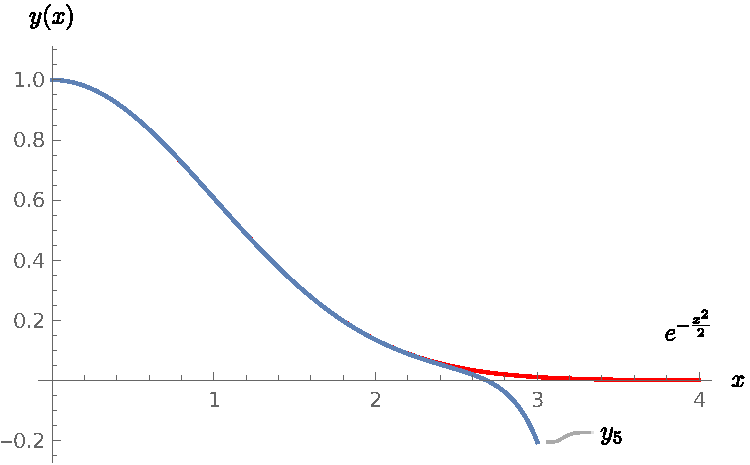
\includegraphics{img/exp_reseni.pdf}
    \caption{Srovnání přesného řešení a páté iterace $y_5$.}
\end{figure}




\subsection{Základní pojmy spektrální analýzy}

Budeme zkoumat operátorovou rovnici pro neznámé $x\in X$
\begin{equation}
    ( \map T -\lambda \Id)x=u\quad,\lambda\in \C,\;  \map T \in \lin(x),\;u\in X \text{ Banachův prostor}
    \label{eq:zadani_vlCisla}
\end{equation}
Motivací k tomu je předchozí paragraf. Označme $ \map T_\lambda\coloneqq  \map T -\lambda\Id$, pak $ \map T_\lambda\in \lin(X)\Leftrightarrow  \map T \in \lin(X)$.

Označme obor hodnot (range) operátoru $ \map T_\lambda$
$$ \mathcal{R}( \map T_\lambda)\coloneqq \{y\in X,\; \exists x\in X,\; \map T_\lambda x=y\}\quad (= \map T_\lambda (X)).$$

Otázky řešitelnosti rovnice (\ref{eq:zadani_vlCisla}) lze přeformulovat v řeči operátoru $ \map T_\lambda$ následovně.
\begin{table}[h!]
    \centering
    \begin{tabular}{c|c}
         V řeči rovnic& V řeči operátoru  \\ \hline\hline
         $\exists$ řešení pro libovolnou pravou stranu $u\in X$? & Je $ \map T_\lambda$ \uu{na}, tj je $ \mathcal{R}( \map T_\lambda)=X$?\\ \hline
         Pokud řešení pro dané $u\in X$ existuje, je určeno jednoznačně? & Je $ \map T_\lambda$ \uu{prostý} na $X$?\\ \hline
         Pokud $\forall u \in \mathcal{R}( \map T_\lambda)\exists! x\in X;\;  \map T_\lambda x=u$, \\je toto řešení \uu{stabilní}? (viz porn. níže)& Je-li $ \map T_\lambda$ prostý, je potom $ \map T_\lambda^{-1}$ spojitý na $\mathcal{R}( \map T_\lambda)$?
    \end{tabular}
\end{table}

\Poznamka 

Pod pojmem \uu{stabilní řešení} míníme (zjednodušeně) situaci, kdy v rovnici $ \map T_\lambda x=u$, která má jednoznačně určená řešení pro $\forall u\in \mathcal{U}(u_0)$ platí, že \uv{malé změny $u\in \mathcal{U}(u_0)$} mají za následek \uv{malé změny řešení}. To přesně odpovídá situaci, kdy je inverzní zobrazení $ \map T_\lambda^{-1}$ spojité na $\mathcal{U}(u_0)$. Tato vlastnost je velmi důležitá při hledání přibližného řešení. Při něm často aproximujeme pravou stranu $u$ nějakou \uv{jí blízkou pravou stranou} $\overline{u}$ a doufáme, že i řešení $\overline{x}$, které odpovídá pravé straně $\overline{u}$, bude blízké řešení $x$, odpovídajícímu pravé straně $u$. Pro \uu{nestabilní} operátory to však nemusí být pravda.

\subsubsection{Podívejme se nejprve na situaci pro $\dim X=n\in \N$.}

V konečné dimenzi je $ \map T \in \lin(X)\Leftrightarrow \exists$ matice $M\in \mathcal{M}^{n\times m}$ taková, že $ \map T (x)=Mx \;\;\forall x \in X$ (v $X$ volíme jednu pevnou bázi).

Potom platí 
%$$ Tady je někde chyba! Když se spustí, nekompiluje se
%\begin{split}
% \map T  \text{ je prostý } &\Leftrightarrow   \map T  \text{ je \uu{na} } \;\;\Leftrightarrow \;\;\; \underbrace{M \text{ reprezentující  \map T  \text{ je regulární.}}}_{ \Updownarrow}  \\  
% \map T ^{-1} \text{ je prostý } &\Leftrightarrow  \map T ^{-1} \text{ je na} \Leftrightarrow \overbrace{M^{-1} \text{ je regulární a reprezentuje }  \map T ^{-1} }\text{ (tj }  \map T ^{-1} \text{ je lin. )}
%\end{split}
%$$


Protože v konečné dimenzi je každý lineární operátor spojitý, je i $ \map T ^{-1}\in\lin(X)$.

V konečné dimenzi tedy platí \uv{všechno nebo nic}, tzn konečně dimenzionální Fredholmova alternativa pro $ \map T \in\lin(X);\;\dim X=n$.

platí právě jedna z násludujících situací:
\begin{enumerate}
    \item $ \map T $ je prostý, na a má spojitou inverzi
    \item $ \map T $ není prostý, není na a nemá spojitou inverzi
\end{enumerate}
\uu{V nekonečné dimenzi} není obecně žádný vztah mezi \uu{prostotou} a zobrazením \uu{na}.

\Priklad

Definujme prostor posloupností $l_2$
$$L_2\coloneqq \Big\{ \{x_n\}_{n=1}^\infty,\; x_n\in\C;\;\sum\limits_{n=1}^\infty|x_n|^2<\infty\Big\}$$

Lze ukázat, že $l_2$ s normou $||\{x_n\}||^2_{l_2}\coloneqq \sum_{n=1}^\infty|x_n|^2$ je Banachův prostor (je dokonce Hilbertův, více později). Na $l_2$ definujme dva tzv. \uu{operátory posunu} (\uv{shift operators})
\begin{equation*}
\begin{split}
  A_1&: (x_1,x_2,x_3,\dots)\mapsto (0,x_1,x_2,x_3,\dots)\\
  A_2&: (x_1,x_2,x_3,\dots)\mapsto (x_2,x_3,x_4,\dots).
\end{split}
\end{equation*}

Evidentně
\begin{equation*}
\begin{split}
  ||A_1x||_{l_2}=||x||_{l_2}&\Rightarrow ||A_1||=\sup\limits_{||x||\leq1}||A_1 x||=1\\
  ||A_2x||_{l_2}=||x||_{l_2}&\Rightarrow ||A_2||\leq1,
\end{split}
\end{equation*}
tedy oa jsou omezené, tedy spojité, tedy $A_1,A_2\in \lin(L_2)$.

Přitom \begin{itemize}
    \item $A_1$ je \uu{prosté} (různým prvkům přiřadí různé prvky, ale není \uu{na} (nic se nezobrazí např. na $(1,0,0,\dots)$
    \item $A_2$ je \uu{na}, ale \uu{není prostý} (rozmyslete).
\end{itemize}

Nicméně, co se týče \uu{stability}, tak i v nekonečné dimenzi platí tato hluboká věta:
\begin{theorem}[O spojitosti inverze bijektivního zobrazení]
\label{theorem:str23}
Nechť $X$ je Banachův prostor, $\map A\in \lin (X)$ je \uu{prosté} a \uu{na}. Potom $\map A^{-1}\in \lin (X)$, speciálně  $\map A^{-1}$ je spojité.
\end{theorem}

\begin{proof}
Plyne z věty o otevřeném zobrazení. Viz \textsc{Lukeš 4.13-4.16}.
\end{proof}

%Tímto se zdá, že problém \uu{stability} řešení je vyřešen: stačí \uu{prostora} a \uu{na}. Ano, pro lineární omezené (tj. spojité operátory tomu tak je. Ale např, pro lineární a nespojité, nebo pro nelineární operátory není situace tak jednoduchá.
    
\subsubsection{Možné stavy operátoru}
Buď $ \map T \in\lin(X)$, $X$ je Banachův, $\lambda\in\C,\;  \map T_\lambda\coloneqq  \map T -\lambda\Id \in\lin(X)$. Pak v závislosti na $\lambda\in\C$ může operátor $ \map T_\lambda$ mít různé vlastnosti z hlediska jeho prostoty, spojitosti inverze a velikosti $\mathcal{R}( \map T_\lambda)$. Následující tabulka shrnuje všechny možnosti, přičemž dvě z nich nemohou nastat: ta, která je vyloučena větou \ref{theorem:str14} (označeno \uv{V1}) a ta, která je vyloučena lemmatem \ref{lemma1}, které zformulujeme a dokážeme za níže (označeno \uv{L1}).

Tabulku je nutno chápat tak, že pomocí ní definujeme různé kategorie, do kterých může patřit parametr $\lambda\in\C$. Tedy např. levý horní roh tabulky je nutno číst takto: \uv{$\lambda\in\C$ je regulárním bodem $ \map T $, pokud $ \map T_\lambda$ je prosté, $ \map T_\lambda^{-1} $ spojité a $\mathcal{R}( \map T_\lambda)=X$}.

\begin{table}[h!]
    \centering
    \begin{tabular}{c||c|c|c}
         & $\overbrace{\mathcal{R}( \map T_\lambda)=X}^{ \map T_\lambda \text{ je \uv{na}}}$   &  $\overbrace{\mathcal{R}( \map T_\lambda)\neq X,\; \overline{\mathcal{R}( \map T_\lambda)}=X}^{ \map T_\lambda \text{ není \uv{na} }}$ &  $\overbrace{\overline{\mathcal{R}( \map T_\lambda)}\neq X}^{ \map T_\lambda \text{ není \uv{na} }}$ \\ \hline\hline
         $ \map T_\lambda \text{ prostý} \big\{ \exists  \map T_\lambda^{-1}$ a je spojitý & $\lambda$ je regulární bod $ \map T $ &  \diagbox{$L1$} &$\lambda\in\Sp_R( \map T )$ \\ \hline
         $ \map T_\lambda \text{ prostý}\big\{\exists  \map T_\lambda^{-1}$ a není spoj. & \diagbox{$V1$} &  $\lambda\in \Sp_C( \map T )$ &$\lambda\in\Sp_R( \map T )$  \\ \hline
         $ \map T_\lambda \text{ není prostý}\big\{\nexists  \map T_\lambda^{-1}$ & $\lambda\in\Sp_P( \map T )$ &  $\lambda\in\Sp_P( \map T )$ &$\lambda\in\Sp_P( \map T )$  \\
    \end{tabular}
    \caption{Spektrální tabulka pro lineární omezené operátory v nekonečné dimenzi.}
    \label{tab:spektra}
\end{table}

\begin{remark}
\begin{itemize}
    \item $\Sp_C(\map T)$ \dots tzv. \uu{spojité spektrum} operátoru $ \map T $. Pokud $\lambda\in \Sp_C(\map T)$, tak rovnice $\map T_\lambda y=u$ nemá řešení pro každou pravou stranu $u\in X$ a každému $\epsilon>0$ existuje $u_\epsilon\in X$, $||u_epsilon-u||_X<\epsilon$ a přitom existuje řešení rovnice $\map T_\lambda y=u_\epsilon\in X$ (to je důsledek toho, že $\overline{\mathcal{R}( \map T_\lambda)}=X$). Někdy se jim říká \uv{skorořešení}. Zároveň však $ \map T_\lambda$ je nestabilní ($ \map T_\lambda^{-1}$ je nespojitý), takže nedává dobrý smysl se bavit o tom, co se děje s řešeními, když trochu měníme pravé strany $u_\epsilon$.
    \item $\Sp_R( \map T )$ \dots tzv. \uu{reziduální spektrum}  $\map T$ . Protože $\overline{\mathcal{R}(\map T_\lambda)}\neq X$, nejsou k dispozici řešení pro velkou část $u\in X$
    \item $\S_P$ \dots tzv. \uu{bodové spektrum} $ \map T $. $ \map T_\lambda$ není prostý, tj. 
    $$\exists x_1\neq x_2,\;  \map T_\lambda x_1= \map T_\lambda x_2 $$
    def. $x\coloneqq x_1-x_2\neq 0$, tj. $\exists x\neq 0$ tak, že 
    \begin{equation*}
    \begin{split}
        \map T_\lambda x &=0 \\
        (\map T -\lambda\Id)x&=0\\
        \map T x&=\lambda x.
    \end{split} 
    \end{equation*}
    
\end{itemize}
\end{remark}


Tedy $\lambda\in\Sp_P(\map T) \Leftrightarrow \exists x\neq 0:\; \map Tx = \lambda x \xLeftrightarrow{\text{def.}} \uu{\lambda\text{ je vlastní číslo }T}$ a $x\neq0$ je odpovídající vl. vektor.

\begin{definition}[Spektrum operátoru]
Nechť $X$ je Banachův prostor a $\map T \in \lin(X)$. Množinu $$ \Sp(\map T)\coloneqq \Sp_C(\map T)\cup \Sp_R(\map T) \cup \Sp_P(\map T)$$ nazýváme spektrem operátoru $\map T$.
\end{definition}


\uu{Pozorování:}
\begin{itemize}
    \item $\lambda\in \Sp(\map T)\Leftrightarrow \map T_\lambda$ není prostý nebo není na
    \item $\lambda$ regulární $\Leftrightarrow \map T_\lambda$ prostý, na (a pak už $\map T_\lambda^{-1}$ spojitý
    \item Ne každý prvek spektra $T$ je vlastním číslem.
\end{itemize}

\begin{definition}[Spektrální poloměr]
Nechť $X$ je Banachův prostor a $\map T \in \lin(X)$. Spektrální poloměr operátoru $\map T$ definujeme předpisem $$ \rho(\map T)\coloneqq \sup \left \lbrace |\lambda|;\; \lambda\in\Sp(\map T) \right \rbrace \:.$$
\end{definition}

\uu{Pozorování:} Pokud je $\rho(\map T) <\infty$, pak platí $|\lambda|>\rho(\map T)\Rightarrow \lambda$ regulární.

Konečně se dostáváme ke slíbenému lemmatu ze spektrální tabulky.
\begin{lemma}[O nespojitosti inverze hustě definovaného injektivního operátoru]
Nechť $X$ je Banachův prostor, $\map A \in \lin (X)$. Nechť dále platí \begin{enumerate}
    \item $\mathcal{R}(\map A)\neq X$, $\overline{\mathcal{R}(\map A)}=X$,
    \item existuje $\map A^{-1}$ a $\mathcal{R}(\map A^{-1}) \mapsto X$ (tj. $\map A$ je prostý na $X$).
\end{enumerate}
Pak $\map A^{-1}$ není spojitý.
\end{lemma}

\begin{proof}
    Pro spor předpokládejme, že $\map A^{-1}$ je spojitý na $\mathcal{R}(\map A)$. Díky vlastnosti $\mathcal{R}(\map A) \neq X$ můžeme zvolit $y\in X\backslash \mathcal{R}(\map A) $ a díky vlastnosti $\overline{\mathcal{R}(\map A)}=X$ existuje posloupnost $\sequence{y_n}{n} \subset \mathcal{R}(\map A)$ taková, že $y_n \rightarrow y$. Navíc díky $\overline{\mathcal{R}(\map A)}=X$ umíme najít i posloupnost $\sequence{x_n}{n} \subset \mathcal{R}(\map A)$ takovou, že $\map A x_n = y_n$, což lze díky existenci inverze psát jako $x_n = \map A^{-1} y_n$. Díky spojitosti $\map A^{-1}$ a cauchoyvskosti $\sequence{y_n}{n}$ je posloupnost $\sequence{x_n}{n}$ cauchyovská. Díky úplnosti prostoru $X$ tato posloupnost konverguje, označme limitní prvek $x$. Pak díky linearitě a spojitosti $\map A$ můžeme psát \begin{align*}
        \map Ax=A(\lim\limits_{n\rightarrow \infty} x_n)\overset{\map A \text{ spoj.}}{=} \lim\limits_{n\rightarrow \infty} \map A x_n = \lim\limits_{n\rightarrow \infty} y_n= y
    \end{align*}
    Protože $\exists x\in X,\; \map Ax=y$, je $y\in\mathcal{R}(\map A)$, což je spor s prvním (podtrženým) bodem.
    
  %  \begin{itemize}
   %     \item $\overline{\mathcal{R}(\map A)}=X \Rightarrow \exists y_n\in\mathcal{R}(\map A);\; y_n\rightarrow y$ v $X$.
%        \item $y_n\in\mathcal{R}(\map A) \Rightarrow \exists x_n\in X, \;\map A(x_n)=y_n \Rightarrow x_n=\map A^{-1}(y_n)$
%        \item $y_n\in\mathcal{R}(\map A)\Rightarrow \exists x_n\in X,\; \map A(x_n)=y_n \Rightarrow x_n=\map A^{-1}(y_n)$
%        \item $y_n$ konverguje v $X \Rightarrow y_n$ je Cauchyovská v $X \xRightarrow{A^{-1} \text{ spoj.}} x_n \text{ je Cauchyovská v } X \xRightarrow{X \text{ úplný}} \exists x\in X$, že  $x_n\rightarrow x$.
%        \item Potom ale
%    \end{itemize}
\end{proof}

\begin{remark}[Tabulka \ref{tab:spektra} v konečné dimenzi]

Víme, že $\map T\in \lin(X);\; \dim X=n\in \N$ je reprezentován maticí $M\in \mathcal{M}^{n\times n}$.

Potom platí:
\begin{equation*}
\begin{split}
    \map T \text{ je prostý }&\Leftrightarrow \map T \text{ je \uu{na} }\quad \Leftrightarrow\quad \;\; \underbrace{M \text{ je regulární}}_{\Updownarrow} \text{ a reprodukuje } \map T \\
   \map T^{-1}\text{ je prostý }&\Leftrightarrow \map T^{-1} \text{ je na }\Leftrightarrow M^{-1} \overbrace{\text{ je regulární}} \text{ a reprezentuje }\map T^{-1}
\end{split}
\end{equation*} 
Za výše popsané situace je navíc vždy i $\map T^{-1}\in\lin(X)$.

Tabulku \ref{tab:spektra} tedy lze schematicky upravit do tvaru
\begin{table}[h!]
    \centering
    \begin{tabular}{c||c|c|c}
    & & & \\\hline\hline
        & \circled{1}& \circled{2},\circled{3} & \circled{4} \\ \hline
        & \circled{2}&\circled{3},\circled{4} & \circled{4} \\ \hline
        & \circled{4}& \circled{3} & \circled{1}
    \end{tabular}
    \caption{Tabulka \ref{tab:spektra} přepsaná v konečné dimenzi}
    \label{tab:spektra_konecnaDim}
\end{table}

\begin{enumerate}[label=\protect\circled{\arabic*}]
\item V \uu{konečné dimenzi} nastává pouze tato situace, a tedy zde máme              
    \begin{enumerate}[label=\arabic*.]
        \item $\lambda\in\C\rightarrow \lambda$ je buď regulární nebo už je to vl. číslo
        \item $\Sp(\map T)=\{ \lambda\in\C,\lambda$ je vlastní číslo $\map T\}=\{\lambda\in\C;\;\lambda$ je vl. číslo $M \}$.
    \end{enumerate}
\item Nemůže obecně nastat
\item Tento sloupec popisuje situaci $\mathcal{R}(\map T_\lambda)\neq X,\; \overline{\mathcal{R}(\map T_\lambda)}=X$. Ta však v konečné dimenzi nastat nemůže, protože v ní platí $\mathcal{R}(\map T_\lambda) = \overline{\mathcal{R}(\map T_\lambda)}$
\item Fourth item
\end{enumerate}

\end{remark}

Následující věta ukazuje, že $\rho(\map T)$ je pro $\map T \in \lin(X)$ vždy konečný.
\begin{theorem}
\label{theorem:str26}
    $X$ Banachův, $T\in \lin(X)$ (tj. $||T||<\infty$). Potom pro $|\lambda|>||\map T||$ platí

\begin{align*}
        &\circled{A}:\;\; \lambda \in \Sp(\map T)\text{, tj. } \lambda \text{ je regulární}  \\
        &\circled{B}:\;\; (T-\lambda\Id)^{-1}=T_\lambda^{-1}=-\sum\limits_{k=0}^\infty\frac{T^k}{\lambda^{k+1}}\in\lin(X) 
\end{align*}
\end{theorem}

\Poznamka \begin{itemize}
    \item Z \circled{A} ihned plyne $\rho(\map T) \leq ||T||$.
    \item Řada v \circled{B} se nazývá von Neumannova řada operátoru $\map T-\lambda \Id)$
\end{itemize}
\begin{proof}
    Je-li $|\lambda|>||\map T||$, pak ještě $\lambda\neq0$. Položme $\map A\coloneqq\frac{1}{\lambda}\map T$. Potom $||\map A||=\frac{1}{|\lambda|}||\map T||<1$ a na $\map A$ můžeme použít větu \ref{theorem:str14}. To nám dá, že:
    \begin{enumerate}[label*=.]
        \item[\circled{A}] $\Id-\map A$ je prostý a na $\Rightarrow \map T-\lambda\Id=(-\lambda)(\Id-\map A$ je prostý a na $\xRightarrow{\text{ věta \ref{theorem:str14}}} (\map T-\lambda\Id )^{-1}$ je spojitý. Odtud je $\lambda$ regulární atd.
        \item[\circled{B}] Věta \ref{theorem:str14} dá i 
        \begin{align*}
            (\Id-\map A)^{-1}&=\sum_{k=0}^\infty \map A^k\\
            (\Id-\frac{1}{\lambda} T)^{-1}&=\sum_{k=0}^\infty\frac{\map T^k}{\lambda^k} \Big/ \cdot (-1)\\
            \left(\frac{1}{\lambda}\map T-\Id \right)^{-1}&=-\sum_{k=0}^\infty\frac{\map T^k}{\lambda^k} \Big/\cdot \frac{1}{\lambda} \quad pozor!\footnotemark\\
            \underbrace{\lambda^{-1}\left(\frac{1}{\lambda}\map T-\Id \right)^{-1}}_{(\map T-\lambda \Id)^{-1}}&=-\sum_{k=0}^\infty\frac{T^k}{\lambda^{k+1}}
        \end{align*}
      \end{enumerate}
    \footnotetext{Inverzní zobrazení k y=3x je y=x/3, tedy inverzní robrazení má hodnotu koeficientu převrácenou. Na levé straně rovnosti lze tedy (alternativně) postupovat:
           $$ \left( \frac{1}{\lambda} \map T-\Id \right)^{-1}=\lambda (T-\lambda \Id)^{-1} \,, $$
           a pak je jasné, proč musíme rovnici dělit $lambda$.}
\end{proof}

\Priklad 
Uvažujme $l_2\coloneqq \left \{ \{x_n\}_{n=1}^\infty,\; x_n\in\C,\;\sum\limits_{n=1}^\infty|x_n|^2<\infty \right \}$ prostor všech komplexních posloupností, které jsou tzv. \uv{sčítatelné s kvadrátem}. Platí, že $l_2$ se skalárním součinem $\innerprod{\{x_n\}}{\{y_n}\}_{l_2}=\sum\limits_{n=1}^\infty x_n\conj{y_n}$ (který indukuje normu $||\{x_n\}_{l_2}=\sqrt{\sum_{n=1}^\infty}|x_n|^2$) je úplný, a tedy Hilbertův (tj. i Banachův) prostor.

Uvažujme operátor 
\begin{align*}
    \map T&:l_2\rightarrow l_2\\
    \map T&:(x_1,x_2\dots,x_k,x_{k+1},\dots)\mapsto (0,x_1,x_2,\dots,x_{k-1},x_k,\dots).
\end{align*}
Protože $||\map T x ||_{l_2}=||x||_{l_2}$, je $||\map T||=\sup\limits_{||x||\leq1}||\map Tx||=\sup\limits_{||x||\leq1}||x||=1$.

Tedy $\rho(\map T)\leq ||T||=1$, a proto $|\lambda|>1\Rightarrow \lambda$ je regulární. Celé spektrum $\map T$ tedy leží v jednotkovém kruhu v $\C$.

\begin{itemize}
    \item $\lambda=0$: Už víme, že $\map T$ \uu{není na}, je prostý. Zároveň je vidět, že žádný prvek z $l_2$ se pomocí $\map T$ nezobrazí na $(a,0,0,\dots)$, $a\in\C,\; a\neq 0$. Nelze tedy žádnou posloupností z $\mathcal{R}(\map T)$ dokonvergovat např. k prvku $(1,0,0,\dots$). Proto $\overline{\mathcal{R}(\map T)}\neq l_2$, odkud plyne $0\in \Sp_R(\map T)$ (plyne z tabulky \ref{tab:spektra}). 
    \item $|\lambda|\leq 1,\; \lambda\neq 0$
\end{itemize}

\begin{enumerate}
    \item Ukážeme nejprve, že žádné z těchto $\lambda$ není vlastním číslem $\map T$. Pokud by tomu tak bylo, tak $\exists x\neq0$, že
    \begin{align*}
        \map T x&=\lambda x\\
        (0,x_1,x_2,\dots)&=(\lambda x_1,\lambda x_2,\dots),
    \end{align*}
    tj. \begin{enumerate}
        \item[i)] $\lambda x_1=0$
        \item[ii)] $\lambda x_k=x_{k-1} \quad \forall k=2,3,4,\dots$
    \end{enumerate}
    Z i) plyne $x_1=0$ (neboť $\lambda\neq 0$), z ii) pak indukcí plyne $x_2=x_3=\dots=0$. Tedy $x=0$, což je však spor s tím, že by to měl výt vlastní vektor $\map T$.
    \item Ukážeme, že $\map T_\lambda$ \uu{není na}, speciálně, že žádné $x\in l_2$ se nezobrazí na $(1,0,0,\dots)$. Nechť takové $x\in l_2$ existuje. Pak tedy
    \begin{align*}
        \underset{\rotatebox[origin=c]{90}{=}}{\map T_\lambda x} &= (1,0,0,\dots),\\[-7pt]
        (-\lambda x_1,x_1-\lambda x_2,&x_2-\lambda x_3,\dots )
    \end{align*}
\end{enumerate}
tedy $1=-\lambda x_1 \Rightarrow x_1=-\frac{1}{\lambda}$

\begin{align*}
    k=1,2,3,\dots \quad x_k-\lambda x_{k+1}=0 \;\Rightarrow\; x_{k+1}=\frac{x_k}{\lambda} \;\Rightarrow\; x=\left(-\frac{1}{\lambda},-\frac{1}{\lambda^2},-\frac{1}{\lambda^3},\dots\right)\\
\end{align*}
Zdánlivě jsme tedy takové $x$ našli, ale $$ ||x||_{l_2}^2=\sum\limits_{k=1}^\infty\frac{1}{\lambda^{2k}}=\infty,$$
neb jde o geometrickou řadu s kvocientem $1/\lambda^2$, pro který $|\lambda|\leq 1 \Rightarrow |1/\lambda^2|\geq 1$.
Protože $\map T_\lambda$ je lineární a $(1,0,0,\dots)\notin \mathcal{R}(\map T_\lambda)$, tak platí také $(a,0,0,\dots \notin \mathcal{R}(\map T_\lambda)\; \forall a \in \C,\;a\neq0\;\Rightarrow\;\overline{\mathcal{R}(\map T_\lambda)}\neq l_2$.

Pohybujeme se tedy v posledním sloupci tabulky \ref{tab:spektra}, $\forall \lambda \neq0,\; |\lambda|\leq1$. Protože však současně žádné takové $\lambda$ není vlastním číslem, je $\lambda \in \Sp_R(\map T)$ pro všechna taková $\lambda$. \footnote{To by šlo také nezávisle ukázat tak, že bychom ukázali prostotu $\map T_\lambda$. Zkuste si.)}

\cc{Závěr}: Pro toto $\map T$ platí $\Sp(\map T)=\Sp_R(\map T)=\{ \lambda\in\C,|\lambda|\leq1\}$. Spektrum je tedy právě celý jednotkový kruh, je tedy nespočetně mnoho prvků spektra (a přitom žádný z nich není vl. číslem). Takový operátor je tedy \uv{poměrně nehezký}, ale přitom negeneruje žádné vl. vektory.

\Cviceni

Zkuste spektrálně analyzovat
\begin{enumerate}[a)]
\item Mějme operátor $\map T: l_2\rightarrow l_2$

      $\quad\qquad (x_1,x_2,x_3,\dots)\mapsto \left(x_2,\frac{x_3}{2},\frac{x_4}{3},\frac{x_5}{4},\dots\right)$
      Zkuste navíc rozmyslet, jaká je $||T||$.
      
      
    \textcolor{gray}{\uu{Řešení:} $\map T\in \lin(l_2), \; \Sp(\map T)=\Sp_P(\map T=\{0\},\; \Sp_R(\map T)=\emptyset,\; \Sp_C(\map T)=\emptyset $}
   
   \item Mějme operátor $\map T: l_2\rightarrow l_2$

      $\quad\qquad (x_1,x_2,x_3,\dots)\mapsto \left(0,x_1,\frac{x_2}{2},\frac{x_3}{3},\frac{x_4}{4},\dots\right)$
Zkuste navíc rozmyslet, jaká je $||T||$ a zda $0\in \Sp_C(\map T)$, nebo $0\in \Sp_R(\map T)$.
      
      
    \textcolor{gray}{\uu{Řešení:} $\map T\in \lin(l_2), \; \Sp(\map T)=\{0\},\; \Sp_P(\map T)=\emptyset,\; \Sp_C(\map T)=\emptyset $}
\end{enumerate}







\pagebreak